\documentclass[11pt,a4paper]{article}
\usepackage[margin=2.2cm]{geometry}
\usepackage{booktabs}
\usepackage{array}
\usepackage{amsmath}
\usepackage{xcolor}
\usepackage{tikz}
\usetikzlibrary{arrows.meta,positioning}
\usepackage{pgfplots}
\pgfplotsset{compat=1.16}
\usepackage{float}
\setlength{\intextsep}{7pt}
\setlength{\textfloatsep}{7pt}
\usepackage{listings}
\usepackage{caption}
\captionsetup{font=small}
\usepackage[hidelinks]{hyperref}

% one colour per mechanism, the same in every graph
\definecolor{cThreads}{HTML}{2A78D6}
\definecolor{cPipes}{HTML}{EB6834}
\definecolor{cShm}{HTML}{1BAF7A}
\definecolor{cMuted}{HTML}{898781}
\definecolor{cGrid}{HTML}{E1E0D9}
\definecolor{cAxis}{HTML}{B4B3AA}
\definecolor{cInk}{HTML}{52514E}
\definecolor{codebg}{RGB}{246,246,244}

\lstset{
  language=C++,
  basicstyle=\ttfamily\footnotesize,
  backgroundcolor=\color{codebg},
  frame=single,
  framerule=0pt,
  breaklines=true,
  columns=fullflexible,
  keepspaces=true,
  showstringspaces=false,
  xleftmargin=4pt,
  aboveskip=6pt, belowskip=4pt,
  tabsize=4
}

\pgfplotsset{
  report/.style={
    width=0.97\textwidth, height=6.6cm,
    axis lines=left, axis line style={cAxis, line width=0.5pt}, tick style={cAxis, line width=0.5pt},
    tick label style={font=\small, text=cInk}, label style={font=\small, text=cInk},
    ymajorgrids, grid style={cGrid, line width=0.4pt},
    legend style={at={(0.5,1.03)}, anchor=south, legend columns=-1, draw=none, fill=none, font=\small,
                  /tikz/every even column/.append style={column sep=10pt}},
    legend cell align=left,
    every axis plot/.append style={line width=1.3pt, mark size=2.3pt, line join=round, line cap=round},
    clip=false,
  },
  threads/.style={cThreads, mark=*, mark options={solid, fill=cThreads, draw=white, line width=0.6pt}},
  pipes/.style={cPipes, mark=square*, mark options={solid, fill=cPipes, draw=white, line width=0.6pt}},
  shm/.style={cShm, mark=triangle*, mark options={solid, fill=cShm, draw=white, line width=0.6pt}, mark size=2.9pt},
  reference/.style={cMuted, line width=0.9pt, mark=none},
}
\tikzset{endlabel/.style={font=\scriptsize, text=cInk, anchor=west, inner sep=2pt}}

% \rows{name} reads the rows of a table from plots/name.tex (written by plots/make_data.py from the measurements)
\makeatletter
\newcommand{\rows}[1]{\@@input plots/#1.tex }
\makeatother
\definecolor{cSockA}{HTML}{EDA100}
\definecolor{cSockB}{HTML}{E87BA4}

\begin{document}

\begin{titlepage}
\centering
\vspace*{1.2cm}
{\large\scshape Operating Systems Laboratory\par}
\vspace{0.3cm}
{\large Laboratory Assignment 5\par}
\vspace{2.4cm}
\rule{\textwidth}{1.2pt}\\[0.55cm]
{\Huge\bfseries Parallel Applications\par}
\vspace{0.35cm}
{\LARGE Threads, Pipes, Shared Memory and Sockets\par}
\vspace{0.55cm}
\rule{\textwidth}{1.2pt}
\vspace{2.6cm}

{\large\bfseries Submitted by\par}
\vspace{0.7cm}
{\large
\begin{tabular}{@{}lcl@{}}
Ayush Yadav       & \quad--\quad & CS24BT001\\[2mm]
Trisham Bepari    & \quad--\quad & CS24BT022\\
\end{tabular}\par}

\vfill
\begin{minipage}{0.88\textwidth}
\small
\noindent\textbf{Abstract.} The image sharpener of Lab~1 (S1 smoothen, S2 find
details, S3 sharpen) was rebuilt as a pipeline whose stages run on different cores and pass their
pixels to each other, in four ways: three threads with a spin lock made of atomic operations, three
processes with pipes, three processes with shared memory and semaphores, and two programs connected
by a TCP socket. Every version writes exactly the image that Lab~1 wrote, for all seven Lab~1
images (143 outputs compared, none different), and a pixel count with an order-dependent hash at
both ends of every link proves that the pixels are received as sent, in the sent order. Passing
every pixel on its own makes all versions 16 to 28 times \emph{slower} than the sequential
baseline: handing a pixel to another core costs 0.5 to 1\,$\mu$s, computing it 35\,ns. Passing
fewer results (variant~2), or the same pixels in larger messages, gives speed-ups of 1.1 to 1.6.
The limit is 1.61 and not 3, because S1 is 62\,\% of the work and a pipeline is as fast as its
slowest stage. For the same reason, giving S1 a computer of its own is the better of the two
partitions in Part~III. Two performance problems that the source code does not show were found
and fixed on the way: false sharing of a cache line, and the address at which the linker places a
function.
\end{minipage}
\vspace{1.2cm}

{\large \today\par}
\end{titlepage}

\section{Setup and Design}

\paragraph{The application.} The image sharpener of Lab~1 has three stages. \textbf{S1} (smoothen)
replaces a pixel by the average of its $3\times3$ neighbourhood, \textbf{S2} (find details) computes
$\max(0,\ \text{input} - \text{smoothened})$ and \textbf{S3} (sharpen) computes
$\min(255,\ \text{input} + \text{details})$, each on the three colour channels. In this assignment the
three stages run at the same time on different cores (Part~II) or on two computers (Part~III), as a
pipeline: a stage does not wait for the previous stage to finish the image, it works on every pixel
as soon as that pixel arrives.

\begin{figure}[H]
\centering
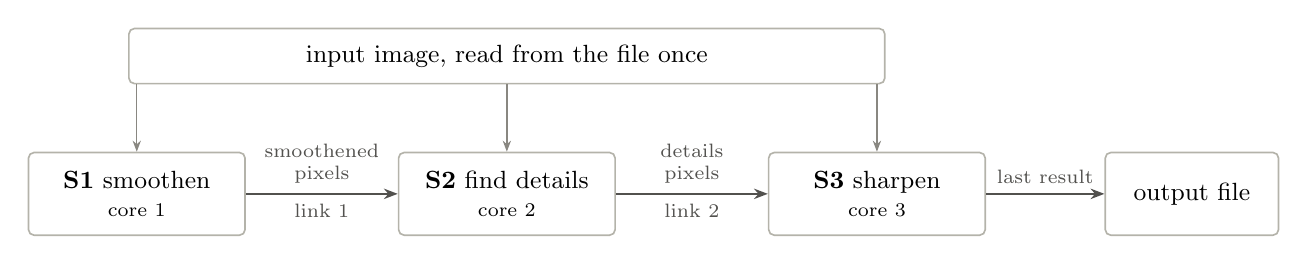
\begin{tikzpicture}[
  box/.style={draw=cAxis, line width=0.6pt, rounded corners=2pt, minimum width=2.75cm, minimum height=1.05cm, align=center, font=\small},
  flow/.style={-{Stealth[length=5pt]}, line width=0.9pt, cInk},
  side/.style={-{Stealth[length=4pt]}, line width=0.5pt, cMuted},
  lbl/.style={font=\scriptsize, text=cInk, align=center}]
\node[box] (s1) at (0,0)    {\textbf{S1} smoothen\\[-1pt]{\scriptsize core 1}};
\node[box] (s2) at (4.7,0)  {\textbf{S2} find details\\[-1pt]{\scriptsize core 2}};
\node[box] (s3) at (9.4,0)  {\textbf{S3} sharpen\\[-1pt]{\scriptsize core 3}};
\node[box, minimum width=2.2cm] (out) at (13.4,0) {output file};
\node[box, minimum width=9.6cm, minimum height=0.7cm] (in) at (4.7,1.75) {input image, read from the file once};
\draw[flow] (s1) -- node[lbl, above] {smoothened\\pixels} node[lbl, below] {link 1} (s2);
\draw[flow] (s2) -- node[lbl, above] {details\\pixels} node[lbl, below] {link 2} (s3);
\draw[flow] (s3) -- node[lbl, above] {last result} (out);
\draw[side] (in.south -| s1) -- (s1.north);
\draw[side] (in.south -| s2) -- (s2.north);
\draw[side] (in.south -| s3) -- (s3.north);
\end{tikzpicture}
\caption{The pipeline. Every stage can read the input image; only the results travel over the two links.}
\label{fig:pipeline}
\end{figure}

\paragraph{What travels over a link.} Only the result of a stage: 3 bytes per pixel, in row-major
order (left to right, top to bottom). No coordinates are sent; the receiver knows which pixel it
got only from its position in the stream. This is why the order matters, and why
Section~\ref{sec:proof} proves that it is kept. All stages also need the input image. Threads share
it, forked processes each get a copy from \texttt{fork()}, and in Part~III computer~A sends it to
computer~B once at the start, so the image file is read exactly once in every program.

\paragraph{Messages.} A link carries \emph{messages} of \texttt{BATCH} pixels. The default is
\texttt{BATCH=1}: every pixel is passed on the moment it is ready, exactly as the assignment asks.
A larger value groups pixels (\texttt{BATCH=450} is one row of our image), which is used in
Section~\ref{sec:results} to study the cost of communication. In both cases the next stage starts
long before the previous one has finished the image.

\paragraph{The two variants.} The transformation is repeated 1000 times on the image that was read
once, to make the experiment compute-intensive.

\begin{table}[H]
\centering\small
\begin{tabular}{@{}llll@{}}
\toprule
& Runs of each stage & Results passed per link & Pixels passed per link \\
\midrule
Variant 1 & 1000 & 1000 (every run) & $1000\times81\,000 = 81$ million \\
Variant 2 & 1000 & 10 (every 100th run) & $10\times81\,000 = 810\,000$ \\
\bottomrule
\end{tabular}
\caption{The two variants do the same amount of computation; variant 2 communicates 100 times less.}
\label{tab:variants}
\end{table}

\noindent In variant~2, S1 passes on only its 100th, 200th, \dots\ run. S2 runs 100 times on every
result it gets: its first run takes the smoothened pixels from the link while S1 is still producing
them, runs 2--100 reuse the copy that S2 kept, and the pixels of the 100th run are passed to S3,
which works the same way. The code is the same for both variants; a stage receives in run $r$ if
$(r-1) \bmod g = 0$ and passes its result on if $r \bmod g = 0$, with $g=1$ in variant~1 and $g=100$
in variant~2. In both variants the image written to the file is the result of the last run of S3,
and since every run starts from the same input image, it must be the image that Lab~1 produced.

\paragraph{Programs.} One self-contained program per part
(Table~\ref{tab:programs}). All of them use the same three functions that process one pixel
(\texttt{S1\_smoothen\_pixel}, \texttt{S2\_find\_details\_pixel}, \texttt{S3\_sharpen\_pixel}), which
are the loop bodies of the Lab~1 functions, unchanged.

\begin{table}[H]
\centering\small
\setlength{\tabcolsep}{5pt}
\begin{tabular}{@{}llll@{}}
\toprule
Program & Workers & Link & Synchronization \\
\midrule
\texttt{part1}    & one thread & -- & -- \\
\texttt{part2\_1} & 3 threads of one process & queue in the address space & spin lock (\texttt{atomic\_flag::test\_and\_set}) \\
\texttt{part2\_2} & 3 processes (\texttt{fork})   & pipe & by the kernel, in \texttt{read}/\texttt{write} \\
\texttt{part2\_3} & 3 processes (\texttt{fork})   & queue in shared memory & two counting semaphores per queue \\
\texttt{part3\_1} & A: S1+S2, \ B: S3 & TCP socket & by the kernel, in \texttt{read}/\texttt{write} \\
\texttt{part3\_2} & A: S1, \ B: S2+S3 & TCP socket & by the kernel, in \texttt{read}/\texttt{write} \\
\bottomrule
\end{tabular}
\caption{The programs. Each takes the variant (1 or 2), and optionally the number of runs and \texttt{BATCH}.}
\label{tab:programs}
\end{table}

\paragraph{Measurements.} All runs were done on an Intel Core i7-8665U laptop (4 cores, 8 hardware
threads), Ubuntu 24.04, \texttt{g++ -O2 -falign-functions=64} (the second flag is explained in
Section~\ref{sec:fair}). The input is image~1 of Lab~1 ($450\times180$, 81\,000
pixels) unless stated otherwise. Times are measured inside the programs with
\texttt{chrono::steady\_clock}. The \emph{processing time} runs from the moment the stages are
started to the moment S3 has finished its last run; reading and writing the files is reported
separately. Every number is the median of 3 to 9 runs, and
\[\text{speed-up} = \frac{\text{processing time of the baseline}}{\text{processing time of the parallel program}}.\]

\paragraph{Building and running.} From \texttt{src/}; every target compiles its program and runs it:
{\small
\begin{verbatim}
make part1                                  # creates output_part1.ppm
make part2_1_variant1                       # also part2_2, part2_3 and variant2
make part2_2_variant1 BATCH=450 RUNS=1000   # optional: pixels per message, runs
make part3_1_variant1_A                     # computer A (waits for B on PORT=12345)
make part3_1_variant1_B HOST=<address of A> # computer B (also part3_2, variant2)
make compare                                # compares all outputs with Lab 1
\end{verbatim}}

\section{Part I: Baseline}

\texttt{part1} is the Lab~1 program with two changes that are needed to run the transformation 1000
times. First, the Lab~1 functions allocated a new image on every call (one \texttt{new} per pixel);
the three images are now allocated once and the functions fill them. Second, the body of each loop
was moved into a function that handles one pixel, so that the parallel programs can call exactly the
same code. The arithmetic is untouched, and with one run the output is identical to the Lab~1 output.
(One line was also added to \texttt{libppm.cpp}: \texttt{read\_ppm\_file} accumulated the width and
height in fields that it never set to zero.)

\begin{table}[H]
\centering\small
\begin{tabular}{@{}lrrrr@{}}
\toprule
Stage & Time for 1000 runs (s) & Range of 8 runs (s) & Per pixel (ns) & Share \\
\midrule
\rows{table_baseline}
\bottomrule
\end{tabular}
\caption{Baseline, image~1: where the time goes. Median of 8 runs; two of them were disturbed by
other activity on the laptop, which is why the upper end of the range is far from the median.}
\label{tab:baseline}
\end{table}

\paragraph{What a pipeline can gain.} Smoothening is 62\,\% of the work, because it reads nine
pixels and divides three times for every pixel it produces, while S2 and S3 need one subtraction or
addition per channel. This limits what three cores can do. The stages run at the same time, but
every pixel still has to pass through S1, and S1 has one core. A pipeline is as fast as its slowest
stage, so with free communication
\[ \text{speed-up} \;\le\; \frac{t_{S1}+t_{S2}+t_{S3}}{\max(t_{S1},\,t_{S2},\,t_{S3})} = \frac{2.86}{1.78} = 1.61, \]
not 3. The same reasoning gives the limits for the two partitions of Part~III: the pipeline is as
fast as the more loaded computer, so \emph{S1+S2 $\vert$ S3} can reach at most
$2.86/(1.78+0.53) = 1.24$ and \emph{S1 $\vert$ S2+S3} at most $2.86/1.78 = 1.61$. These limits are
drawn in the graphs of Section~\ref{sec:results}.

\section{Part II: One Pipeline, Three Mechanisms}
\label{sec:design}

The three programs have the same structure. A stage loops over its runs and over the pixels of the
image; it calls a \emph{receive} function when it reaches a pixel that it does not have yet,
processes the pixel, and calls a \emph{send} function as soon as a message is complete. Only these
two functions, and the way the three workers are created, differ between the programs.

\subsection{Threads and atomic operations (\texttt{part2\_1})}

The three stages are three \texttt{std::thread}s. A link is a queue in the address space of the
process: a circular buffer of 64 message slots with the fields \texttt{head}, \texttt{tail} and
\texttt{count}. The fields are protected by a spin lock made of one \texttt{atomic\_flag}.
\texttt{test\_and\_set()} sets the flag and returns the value it had before, in one atomic step, so
it returns \texttt{false} for exactly one thread: the one that changed the flag from clear to set.
That thread owns the lock until it calls \texttt{clear()}.

\begin{lstlisting}
void send_pixels(struct queue_t *queue, uint8_t *pixels, int number_of_pixels)
{
    while (true)
    {
        while (queue->lock.test_and_set()) {}       // spin until the lock is ours
        if (queue->count < QUEUE_SIZE)
        {
            memcpy(queue->messages + (size_t) queue->tail * batch * 3,
                   pixels, number_of_pixels * 3);
            queue->tail = (queue->tail + 1) % QUEUE_SIZE;
            queue->count++;
            queue->lock.clear();
            return;
        }
        queue->lock.clear();                        // queue full: let the receiver in, try again
    }
}
\end{lstlisting}

\noindent \texttt{receive\_pixels} is the mirror image (it waits while \texttt{count} is 0). Nothing
ever sleeps: a stage that waits for a pixel keeps taking and releasing the lock, so it keeps a core
fully busy. No other synchronization is used.

\paragraph{A false-sharing bug.} The first version passed every test but was strangely slow:
variant~2, which passes only 10 results, took 3.6--4.4\,s, much longer than the baseline. The symbol
table (\texttt{nm}) showed why: the linker had placed the first queue, with its lock, in the same
64-byte cache line as the read-only globals \texttt{input\_image}, \texttt{batch} and \texttt{runs}.
The waiting threads write the lock continuously, so S1 lost that cache line again and again while
it computed, although it only \emph{reads} those globals. Declaring the queue as
\texttt{struct alignas(64) queue\_t} gives each queue a cache line of its own and brought the same
run down to 2.1--2.2\,s. Nothing was wrong with the logic; the program was only slow.

\subsection{Processes and pipes (\texttt{part2\_2})}

The parent reads the image, creates two pipes with \texttt{pipe()} and calls \texttt{fork()} three
times; it then only waits for its children and checks their exit status. A child sends a message
with one \texttt{write()} and receives it with \texttt{read()}. The kernel does all the
synchronization: \texttt{read()} blocks while the pipe is empty and \texttt{write()} blocks while it
is full (a pipe holds 64\,KB by default, about 21\,845 pixels), and a blocked process sleeps without
using a core. Three details needed care:
\begin{itemize}\setlength{\itemsep}{1pt}
\item \emph{Unused ends must be closed} in every process. \texttt{read()} reports the end of the
stream only when \emph{all} copies of the write end are closed, and \texttt{fork()} copies all four
descriptors into all three children.
\item \emph{Short reads and writes.} \texttt{read()} returns as soon as some bytes are available and
\texttt{write()} may write only part of a large message, so both are wrapped in loops
(\texttt{receive\_bytes}, \texttt{send\_bytes}) that continue until the whole message is through.
\item \emph{Anonymous pipes are enough} because the three processes have a common parent. Unrelated
processes would need a FIFO (\texttt{mkfifo}), which behaves in the same way once both ends are open.
\end{itemize}

\subsection{Processes, shared memory and semaphores (\texttt{part2\_3})}

Before forking, the parent creates a POSIX shared memory object (\texttt{shm\_open}, sized with
\texttt{ftruncate}) and maps it with \texttt{mmap(..., MAP\_SHARED, ...)}. The children inherit the
mapping, so all four processes see the same bytes. The name is removed with \texttt{shm\_unlink}
right after the mapping is made: the memory lives on until the last process unmaps it, and nothing
is left behind in \texttt{/dev/shm} even if the program is killed. The object holds two queues like
those of \texttt{part2\_1}, but each is synchronized by two unnamed semaphores that are stored in
the shared memory itself (\texttt{sem\_init} with \texttt{pshared = 1}): \texttt{empty\_slots}
starts at 64 and \texttt{full\_slots} at 0.

\begin{lstlisting}
void send_pixels(struct queue_t *queue, uint8_t *pixels, int number_of_pixels)
{
    sem_wait(&queue->empty_slots);                  // sleeps while the queue is full
    memcpy(queue->messages + (size_t) queue->tail * batch * 3,
           pixels, number_of_pixels * 3);
    queue->tail = (queue->tail + 1) % QUEUE_SIZE;
    sem_post(&queue->full_slots);                   // wakes the receiver if it sleeps
}
\end{lstlisting}

\noindent \texttt{receive\_pixels} is the mirror image: it waits on \texttt{full\_slots}, copies the
message at \texttt{head} out, and posts \texttt{empty\_slots}. This is the bounded buffer from the
lectures without its mutex. The mutex is not needed
here because a queue has exactly one sender and one receiver: \texttt{tail} is touched only by the
sender and \texttt{head} only by the receiver, and the semaphores guarantee that the two never work
on the same slot.

\section{Proof that Pixels are Received as Sent, in the Sent Order}
\label{sec:proof}

\paragraph{Method.} On every link, the sender and the receiver each keep a count of the pixels and
an order-dependent hash of them, the FNV-1a style hash that Lab~4 used for frame numbers. For every
pixel $p$ (its three bytes packed into one number), in the order in which it is sent, respectively
received:
\[ H \leftarrow (H \oplus p) \times 1099511628211 \bmod 2^{64}, \qquad H_0 = 1469598103934665603. \]
When a sender has finished, it hands its count and hash to the receiver's side, and the two pairs are
compared. The sender's pair travels outside the path under test or after it: through the pipe or
socket \emph{after} the last pixel, through fields in the shared memory, or through global variables.
Every program prints, for every link, both pairs and \texttt{PASSED} or \texttt{FAILED}, and returns
a non-zero exit status on a failure.

\paragraph{Why this is a proof.} The receiver hashes the pixels in the order in which \emph{it}
gets them. The hash is a chain: each step multiplies the result of all previous steps, so swapping
two different pixels, changing one bit, losing a pixel or delivering one twice changes the final
value (two different sequences collide with a probability of about $2^{-64}$). A lost or duplicated
pixel also changes the count. Equal counts and equal hashes therefore mean that the receiver got the
same sequence of pixels that the sender sent.

\paragraph{Result.} The check passed in every run we made: in all runs of
Section~\ref{sec:compare} and in all timed runs of Section~\ref{sec:results}, for every link.
Table~\ref{tab:hash} shows the default configuration. The five programs agree with each other as
well: the stream of smoothened pixels has the same hash whether it goes through a queue, a pipe,
shared memory or a socket, and so has the stream of details pixels.

\begin{table}[H]
\centering\small
\setlength{\tabcolsep}{4.5pt}
\begin{tabular}{@{}llrll@{}}
\toprule
Stream & Variant & Sent = received & Hash at sender = at receiver & Same value in \\
\midrule
smoothened (link 1) & 1 & 81\,000\,000 & 12170038745284060307 & \texttt{part2\_1}, \texttt{2\_2}, \texttt{2\_3}, \texttt{3\_2} \\
smoothened (link 1) & 2 & 810\,000     & 16510668365919690495 & \texttt{part2\_1}, \texttt{2\_2}, \texttt{2\_3}, \texttt{3\_2} \\
details (link 2)    & 1 & 81\,000\,000 & 1901646794791207459  & \texttt{part2\_1}, \texttt{2\_2}, \texttt{2\_3}, \texttt{3\_1} \\
details (link 2)    & 2 & 810\,000     & 12032347268811867531 & \texttt{part2\_1}, \texttt{2\_2}, \texttt{2\_3}, \texttt{3\_1} \\
\bottomrule
\end{tabular}
\caption{Counts and hashes printed by the programs (image~1, 1000 runs, \texttt{BATCH=1}).}
\label{tab:hash}
\end{table}

\paragraph{Does the check notice a fault?} A check that always says \texttt{PASSED} proves nothing,
so we broke the link on purpose in copies of the programs (Table~\ref{tab:fault}).

\begin{table}[H]
\centering\small
\begin{tabular}{@{}p{6.9cm}p{4.3cm}p{4.2cm}@{}}
\toprule
Fault injected & Link check & Output file \\
\midrule
Two neighbouring pixels change places on link~1, once, in the first run (pipes) &
\texttt{FAILED}: counts equal, hashes differ & identical to Lab~1 \\
One bit of one pixel is flipped on link~1, once, in the first run (pipes) &
\texttt{FAILED}: counts equal, hashes differ & identical to Lab~1 \\
The spin lock is removed from the queue (threads) &
program never finishes (6 of 6 attempts) & not written \\
\bottomrule
\end{tabular}
\caption{Fault injection. The first two faults are invisible in the output file.}
\label{tab:fault}
\end{table}

\noindent The first two rows are the reason why comparing the output image with the Lab~1 image is
\emph{not} a proof by itself. Only the result of the last run is written to the file, so a pixel
that is lost or misplaced in any of the 999 earlier runs leaves no trace there. The hash covers
every pixel of every run. The output comparison of Section~\ref{sec:compare} is still done, as
independent evidence for the last run.

\section{Run Time and Speed-up}
\label{sec:results}

\subsection{First, a fair comparison}
\label{sec:fair}

All programs contain the same function \texttt{S1\_smoothen\_pixel}, so S1 by itself should take the
same time in each of them. We checked this with a run in which almost nothing is communicated
(variant~2, one whole image per message) and it was \emph{not} true. Built with plain
\texttt{g++ -O2}, S1 needed about 1.55\,s for its 1000 runs in the baseline and in the pipe program,
but 2.3--2.5\,s in the thread program (Table~\ref{tab:align}). Left alone, this would have looked
like a property of threads. We ruled out the obvious explanations one by one:
\begin{itemize}\setlength{\itemsep}{1pt}
\item \emph{Busy waiting?} No. When the two waiting threads slept instead of spinning, S1 was just as slow.
\item \emph{Hyper-threading or a lower clock?} No. The three threads ran on three different physical
cores at about 4.0\,GHz, measured during the run.
\item \emph{The place of the buffers in memory?} No. Moving S1's buffer with allocator settings changed
its address but not the time.
\end{itemize}
\texttt{objdump} then showed that the instructions of the function are identical, byte for byte, in
the thread program and in the pipe program. Only the address at which the linker put the function
differs. On this processor generation the speed of a piece of code depends on where its jump
instructions fall relative to 32-byte boundaries (Intel documents this as the ``jump conditional
code'' erratum), and \texttt{S1\_smoothen\_pixel}, with its nine bounds checks, is mostly jumps. Two
things confirmed it: the assembler option that keeps jumps away from these boundaries removed the
difference, and so did \texttt{-falign-functions=64}, which starts every function at a 64-byte
boundary and therefore gives the function the same layout in every program. All programs are built
with the second flag. S1 then takes the same time everywhere, within the run-to-run variation.

\begin{table}[H]
\centering\small
\begin{tabular}{@{}lcccc@{}}
\toprule
Time for 1000 runs of S1 (s), three runs each & \texttt{part1} & \texttt{part2\_1} & \texttt{part2\_2} & \texttt{part2\_3} \\
\midrule
\texttt{g++ -O2}                         & 1.55--1.92 & 2.28--2.47 & 1.53--1.77 & 1.58--1.78 \\
\texttt{g++ -O2 -falign-functions=64}    & 1.69--1.75 & 1.67--1.79 & 1.61--1.78 & 1.73--1.88 \\
\bottomrule
\end{tabular}
\caption{The same function, placed at different addresses by the linker (top) and at the same
position in every program (bottom).}
\label{tab:align}
\end{table}

\noindent What remains is a run-to-run variation of about $\pm5\,\%$ (it is a laptop: the clock
frequency depends on the temperature and on how many cores are busy), so a difference of a few
percent between two programs below should not be read as significant.

\subsection{Pixel by pixel (\texttt{BATCH=1})}

\begin{table}[H]
\centering\small
\setlength{\tabcolsep}{2.6pt}
\begin{tabular}{@{}ll rrrr rrr@{}}
\toprule
& & \multicolumn{4}{c}{Variant 1 (81 million pixels per link)} & \multicolumn{3}{c}{Variant 2 (810\,000 per link)} \\
\cmidrule(lr){3-6}\cmidrule(l){7-9}
Program & Workers, link & Time (s) & Range (s) & Speed-up & ns/pix. & Time (s) & Range (s) & Speed-up \\
\midrule
\texttt{part1} & one thread (baseline) & 2.86 & 2.58--4.18 & 1 & 35 & 2.86 & 2.58--4.18 & 1 \\
\midrule
\rows{table_main}
\bottomrule
\end{tabular}
\caption{Processing time with every pixel passed on its own (image~1, 1000 runs). Median of 3 runs
(variant~1) or 5 runs (variant~2). ``ns/pixel'' is the time divided by the 81 million pixels that
go through the pipeline. The two socket programs ran as two processes on one computer (Section~\ref{sec:part3}).}
\label{tab:main}
\end{table}

\paragraph{Variant 1 is 16 to 28 times slower than the baseline.} Not one of the five programs
gains anything from its extra cores; the fastest of them needs 45\,s for what the baseline does in
2.9\,s. The reason is in the last column of the left half. The baseline needs 35\,ns to take a pixel
through all three stages. With every pixel handed to another core on its own, a pixel needs 550 to
1000\,ns, however the hand-over is done, so more than 93\,\% of the time goes into passing pixels
and less than 7\,\% into computing them.

\begin{table}[H]
\centering\small
\begin{tabular}{@{}lrrrrrr@{}}
\toprule
& & Elapsed & CPU time in the & CPU time in & Voluntary context & Switches \\
Program & \texttt{BATCH} & time (s) & program (s) & the kernel (s) & switches & per message \\
\midrule
\rows{table_usage}
\bottomrule
\end{tabular}
\caption{Variant~1 with 100 runs of image~1 (8.1 million pixels per link, two links), measured with
\texttt{/usr/bin/time}. A voluntary context switch is a process going to sleep because it has to wait.}
\label{tab:usage}
\end{table}

\paragraph{Three different ways to lose.} Table~\ref{tab:usage} shows where the time goes when every
pixel is a message.
\begin{itemize}\setlength{\itemsep}{1pt}
\item The \emph{thread} program never enters the kernel and never sleeps (11 voluntary context
switches in the whole run), but it uses 11.3\,s of processor time in 3.8\,s: all three cores are
busy all the time. The baseline needs 0.29\,s of processor time for the same computation, so about
97\,\% of the processor time goes into taking and releasing the two spin locks and into waiting.
\item The \emph{pipe} program makes one \texttt{write()} and one \texttt{read()} per message;
\texttt{strace} counted 324\,043 and 324\,037 calls for 324\,000 messages. 82\,\% of its processor
time is spent inside the kernel.
\item The \emph{semaphore} program needs no system call to pass a message as long as nobody is
waiting. But S2 is faster than S1 and keeps catching up with it, so a stage went to sleep 3.25
million times, once every 5 messages. Each time costs a system call to go to sleep, another one to
be woken up and a context switch, and in the end 75\,\% of its processor time is kernel time too.
\end{itemize}
With one row per message (lower half of the table) the kernel time is almost gone. A stage now goes
to sleep for nearly every message (0.97 switches per message), but there are 450 times fewer
messages.

\paragraph{Variant 2 is faster than the baseline in every program.} It does exactly the same
computation but passes 100 times fewer pixels, and the speed-up is 1.18 to 1.38. The two variants
were measured with the same programs and the same code path; the only thing that changed is how
often the stages talk to each other.

\subsection{More pixels per message}

Variant~1 does not have to be slow. The stages only have to stop synchronizing once per pixel.
With \texttt{BATCH}$=n$ a stage collects $n$ pixels and passes them in one message: one lock
acquisition, one \texttt{write()}, or one pair of semaphore operations for $n$ pixels. The next
stage still starts long before the image is finished (an image is 81\,000 pixels).

\begin{figure}[H]
\centering
\begin{tikzpicture}
\begin{axis}[report, width=0.86\textwidth, height=6.5cm, xmode=log, ymode=log,
  xmin=0.75, xmax=110000, ymin=1.5, ymax=110,
  xtick={1,4,16,64,256,1024,4096,16384,81000},
  xticklabels={1,4,16,64,256,1\,024,4\,096,16\,384,81\,000},
  ytick={2,3,5,10,20,50,100}, yticklabels={2,3,5,10,20,50,100},
  xlabel={Pixels per message (\texttt{BATCH}), log scale},
  ylabel={Processing time (s), log scale}]
\addplot[reference, forget plot] coordinates {(0.75,2.862) (110000,2.862)};
\node[endlabel] at (axis cs:110000,2.862) {baseline, 2.86\,s};
\addplot[reference, forget plot] coordinates {(0.75,1.783) (110000,1.783)};
\node[endlabel] at (axis cs:110000,1.783) {S1 alone, 1.78\,s};
\addplot[threads] table[x=batch, y=threads]{plots/batch.dat};
\addlegendentry{threads, atomic operations}
\addplot[pipes] table[x=batch, y=pipes]{plots/batch.dat};
\addlegendentry{processes, pipes}
\addplot[shm] table[x=batch, y=shm]{plots/batch.dat};
\addlegendentry{processes, shared memory}
\end{axis}
\end{tikzpicture}
\caption{Variant~1 (1000 results per link): processing time against the number of pixels per
message. Below the upper grey line a program is faster than the baseline; no pipeline can go below
the lower one, the time that S1 needs alone.}
\label{fig:batch}
\end{figure}

\begin{table}[H]
\centering\small
\setlength{\tabcolsep}{5pt}
\begin{tabular}{@{}lr rr rr rr@{}}
\toprule
& & \multicolumn{2}{c}{Threads} & \multicolumn{2}{c}{Pipes} & \multicolumn{2}{c}{Shared memory} \\
\cmidrule(lr){3-4}\cmidrule(lr){5-6}\cmidrule(l){7-8}
Pixels per message & Messages per link & Time (s) & Speed-up & Time (s) & Speed-up & Time (s) & Speed-up \\
\midrule
\rows{table_batch}
\bottomrule
\end{tabular}
\caption{The data of Figure~\ref{fig:batch}: variant~1, image~1, 1000 runs, median of 3 runs.
The baseline takes 2.86\,s.}
\label{tab:batch}
\end{table}

\paragraph{The time falls in proportion to the number of messages, then stops.} From 1 to 8 pixels
per message every doubling of the message roughly halves the time (pipes: 56.8, 30.2, 16.6,
8.1\,s), which shows that the time was being spent per message and not per pixel. Threads pass the
baseline at about 32 pixels per message, shared memory at about 128 and pipes at about 256. The
order makes sense: taking a spin lock that nobody else holds costs a few nanoseconds, a semaphore
operation costs more and needs the kernel whenever somebody has to be woken up, and a
\texttt{write()} enters the kernel every time.

\paragraph{Beyond about 1000 pixels per message nothing more is gained.} All three programs then
take 2.0 to 2.6\,s, a speed-up of 1.1 to 1.4, and the differences between them are no larger than
the differences between two runs of the same program (for example pipes: 2.23\,s at 4096 pixels,
2.57\,s at 16\,384, 2.28\,s for whole images). Communication has become almost free, and what is
left is the limit of the pipeline itself: the lower grey line. One row of the image per message
(\texttt{BATCH=450}) is already in this region.

\subsection{Where the limit comes from: variant 2 in detail}

\begin{table}[H]
\centering\small
\begin{tabular}{@{}lrrrrr@{}}
\toprule
Program & \texttt{BATCH} & S1 finished after (s) & S2 finished after (s) & S3 finished after (s) & Speed-up \\
\midrule
\rows{table_variant2}
\bottomrule
\end{tabular}
\caption{Variant~2, image~1, 1000 runs: the time after which each stage had finished (median of 5
runs for \texttt{BATCH=1}, of 3 runs for \texttt{BATCH=450}). The baseline needs 1.78\,s for S1 alone.}
\label{tab:variant2}
\end{table}

\paragraph{The pipeline takes exactly as long as S1.} In every row S2 finishes about 0.03\,s after
S1, and S3 about 0.03\,s after S2. That is the time they need for the last result (100 runs take
S2 0.05\,s). So S2 and S3 are not short of time: each of them has work for about 0.5\,s and
spends the other 1.2 to 1.7\,s waiting for S1. Adding more cores to S2 or S3 would change nothing;
only a faster S1 would. With one row per message the programs reach a speed-up of 1.47 to 1.63,
which is the limit of 1.61 within the accuracy of the measurement (the baseline's own S1 took
between 1.63 and 1.82\,s in its undisturbed runs).

\paragraph{Busy waiting is not free.} In both halves of Table~\ref{tab:variant2} the thread program
is the slowest of the three, by 4 to 11\,\%, although its stages do the same work. Its S2 and S3
never sleep; they spin while they wait, so three cores are fully busy for the whole run instead of
one. A control experiment without any pipeline shows the size of this effect: the baseline's S1
took 1.55\,s on a quiet machine, 1.8\,s while two unrelated processes were spinning on two other
cores (most likely because the processor lowers its clock frequency when more cores are active),
and 3.95\,s when a spinning process was placed on the second hardware thread of the same core. A
stage that waits in \texttt{read()} or \texttt{sem\_wait()} sleeps, and costs the working stage
nothing.

\begin{figure}[H]
\centering
\begin{tikzpicture}
\begin{axis}[report, width=0.88\textwidth, height=5.4cm, ybar=1.6pt, bar width=8.5pt,
  xmin=0.45, xmax=4.55, ymin=0, ymax=1.85, xtick={1,2,3,4},
  xticklabels={{variant 1\\pixel by pixel},{variant 1\\one row per message},{variant 2\\pixel by pixel},{variant 2\\one row per message}},
  x tick label style={align=center, font=\small, text=cInk}, x tick style={draw=none},
  ytick={0,0.5,1,1.5}, ylabel={Speed-up over the baseline},
  legend style={at={(0.5,1.04)}, anchor=south, legend columns=3, draw=none, fill=none, font=\small,
                /tikz/every even column/.append style={column sep=10pt}},
  legend image code/.code={\fill[#1] (0cm,-0.09cm) rectangle (0.22cm,0.13cm);}]
\addplot[fill=cThreads, draw=none] table[x=configuration, y=threads]{plots/speedups.dat};
\addlegendentry{threads}
\addplot[fill=cPipes, draw=none] table[x=configuration, y=pipes]{plots/speedups.dat};
\addlegendentry{pipes}
\addplot[fill=cShm, draw=none] table[x=configuration, y=shm]{plots/speedups.dat};
\addlegendentry{shared memory}
\addplot[fill=cSockA, draw=none] table[x=configuration, y=sockets31]{plots/speedups.dat};
\addlegendentry{sockets, S1+S2 $\vert$ S3}
\addplot[fill=cSockB, draw=none] table[x=configuration, y=sockets32]{plots/speedups.dat};
\addlegendentry{sockets, S1 $\vert$ S2+S3}
\draw[cMuted, line width=0.9pt] (axis cs:0.45,1) -- (axis cs:4.55,1);
\node[endlabel] at (axis cs:4.55,1) {baseline};
\draw[cMuted, line width=0.9pt] (axis cs:0.45,1.61) -- (axis cs:4.55,1.61);
\node[endlabel] at (axis cs:4.55,1.61) {limit, 1.61};
\node[font=\scriptsize, text=cInk, anchor=south] at (axis cs:1,0.08) {0.04 to 0.06};
\end{axis}
\end{tikzpicture}
\caption{All five programs in four configurations (image~1, 1000 runs; values in
Tables~\ref{tab:main}, \ref{tab:batch}, \ref{tab:variant2} and \ref{tab:part3}). The limit for
\emph{sockets, S1+S2 $\vert$ S3} is 1.24 instead of 1.61.}
\label{fig:summary}
\end{figure}

\paragraph{Summary of the two variants.} Figure~\ref{fig:summary} puts the results side by side.
The amount of computation is the same in all four groups. Two things differ: the number of
messages per link (81 million, 180\,000, 810\,000 and 1800) and the number of pixels that are moved
at all (81 million in variant~1, 810\,000 in variant~2). The first group pays for 81 million
synchronizations and loses everything. In the second group the synchronizations are gone, but
every pixel is still copied into a message and out of it, and hashed at both ends for the proof;
this is why variant~1 stays below variant~2 even with large messages. (Switching the hash off made
the three programs of Part~II 1 to 8\,\% faster in the second group, so the proof is the smaller
part of that cost.) The picture is the same for threads, pipes, shared memory and sockets.

\subsection{Images of other sizes}

\begin{table}[H]
\centering\small
\setlength{\tabcolsep}{4.2pt}
\begin{tabular}{@{}rlrrrr rrr rrr@{}}
\toprule
& & & \multicolumn{3}{c}{Baseline} & \multicolumn{3}{c}{Speed-up, variant 1} & \multicolumn{3}{c}{Speed-up, variant 2} \\
\cmidrule(lr){4-6}\cmidrule(lr){7-9}\cmidrule(l){10-12}
Image & Size & Mpixel & Time (s) & ns/pixel & $T/t_{S1}$ & Thr. & Pipes & Shm & Thr. & Pipes & Shm \\
\midrule
\rows{table_images}
\bottomrule
\end{tabular}
\caption{The seven images of Lab~1, 100 runs, one row of the image per message, median of 3 runs
(9 for image~1, which was measured separately because its runs last only 0.2\,s).
With 100 runs variant~2 passes a single result, so its stages work one after the other.}
\label{tab:images}
\end{table}

\begin{figure}[H]
\centering
\begin{tikzpicture}
\begin{axis}[report, width=0.86\textwidth, height=5.0cm, xmode=log,
  xmin=0.065, xmax=11.5, ymin=0, ymax=2.3,
  xtick={0.081,0.309,0.589,1.165,1.5,3.41,9.26},
  xticklabels={0.08,0.31,0.59,1.16,,3.4,9.3},
  ytick={0,0.5,1,1.5,2},
  xlabel={Image size (million pixels, log scale)}, ylabel={Speed-up over the baseline}]
\addplot[reference, forget plot] coordinates {(0.065,1) (11.5,1)};
\node[endlabel] at (axis cs:11.5,1) {baseline};
\addplot[threads] table[x expr=\thisrow{pixels}/1000000, y=speedup_threads]{plots/images_v1.dat};
\addlegendentry{threads, atomic operations}
\addplot[pipes] table[x expr=\thisrow{pixels}/1000000, y=speedup_pipes]{plots/images_v1.dat};
\addlegendentry{processes, pipes}
\addplot[shm] table[x expr=\thisrow{pixels}/1000000, y=speedup_shm]{plots/images_v1.dat};
\addlegendentry{processes, shared memory}
\end{axis}
\end{tikzpicture}
\caption{Variant~1, one row per message, 100 runs: speed-up for the seven images.}
\label{fig:images}
\end{figure}

\paragraph{Larger images give larger speed-ups.} For images~2 to 7 the pipeline of variant~1
reaches 1.6 to 1.7 with threads and 1.3 to 1.6 with processes, against 1.2 to 1.4 for image~1. The
baseline becomes slower per pixel (44 to 46\,ns instead of 33\,ns): it keeps four images in which
every pixel is a separate 32-byte block, and from image~2 on these no longer fit into the 8\,MB
cache of the processor. S2 and S3 suffer most, so their share of the work grows and with it the
limit $T/t_{S1}$ of the pipeline, from 1.7 to 1.9.

\paragraph{Not all of the speed-up comes from the three cores.} The right part of
Table~\ref{tab:images} is a control experiment. With 100 runs variant~2 passes one single result,
so S1, S2 and S3 work one after the other and nothing is done in parallel. Nevertheless these runs
are 1.1 to 1.3 times faster than the baseline, for every image. The reason is the data layout: a
stage of the pipeline keeps the pixels it receives in a compact array of 3 bytes per pixel, so its
S2 is about 2.5 times and its S3 1.2 to 2 times faster than those of the baseline, which follow two
pointers for every pixel of every image. A sequential program with compact arrays would gain this factor too.
What the three cores add is the difference between the two halves of the table.

\paragraph{Threads are the fastest on large images.} A likely reason is in Table~\ref{tab:usage}:
with one row per message a sleeping stage is woken up by the kernel for nearly every message, and
waking up takes time; a spinning stage takes the row the moment it is ready. Busy waiting costs
processor time (Section~\ref{sec:results}.4) but no latency.

\subsection{The original experiment: a single run}

\begin{table}[H]
\centering\small
\setlength{\tabcolsep}{3.7pt}
\begin{tabular}{@{}rl rrrrrr rrr rrr@{}}
\toprule
& & \multicolumn{6}{c}{Baseline, one run (ms)} & \multicolumn{6}{c}{Speed-up of the whole run} \\
\cmidrule(lr){3-8}\cmidrule(l){9-14}
& & & Allo- & S1, S2, & & & Stages, & \multicolumn{3}{c}{one row per message} & \multicolumn{3}{c}{pixel by pixel} \\
\cmidrule(lr){9-11}\cmidrule(l){12-14}
Image & Size & Read & cate & S3 & Write & Total & share & Thr. & Pipes & Shm & Thr. & Pipes & Shm \\
\midrule
\rows{table_single}
\bottomrule
\end{tabular}
\caption{The experiment of Lab~1: one run of S1, S2 and S3 (variant~1), median of 5 runs (9 for image~1).
``Allocate'' is the time to create the three result images, one block per pixel.}
\label{tab:single}
\end{table}

\paragraph{With one run, the three stages are a fifth of the work.} The assignment expected the
reading and writing of the files to dominate, and they do: the stages are only 19 to 21\,\% of a
run of the baseline. The rest is reading the file byte by byte (22 to 30\,\%), writing it
(12\,\%) and, the largest part, allocating the three result images with one \texttt{new} per pixel
(39 to 46\,\%). Three cores can only shorten the fifth that the stages take, by a factor of at most
1.6 to 1.9, which would make the whole run about 1.1 times faster.

\paragraph{The measured gain is larger, but it is not parallelism.} With one row per message the
programs finish 1.4 to 1.8 times sooner than the baseline. Most of this comes from something else:
a pipeline stage keeps what it receives in a compact array, so these programs allocate only one
image of per-pixel blocks (the output) instead of three. The stages themselves
took 0.25\,s in the thread program against 0.40\,s in the baseline for image~7. Pixel by pixel, a
single run is 3 to 5 times slower than the baseline, for the reasons given above.

\section{Ease of Implementing and Debugging}

\begin{table}[H]
\centering\small
\setlength{\tabcolsep}{4pt}
\renewcommand{\arraystretch}{1.15}
\begin{tabular}{@{}p{2.5cm}p{4.2cm}p{4.2cm}p{4.6cm}@{}}
\toprule
& Threads + atomic operations & Processes + pipes & Processes + shared memory + semaphores \\
\midrule
Setting up &
Nothing: globals are shared, a queue is a struct. &
\texttt{pipe()} twice, \texttt{fork()} three times, close the unused ends. &
\texttt{shm\_open}, \texttt{ftruncate}, \texttt{mmap}, \texttt{shm\_unlink}, four \texttt{sem\_init}, then \texttt{fork()}. The most code. \\
Synchronization we write &
All of it: the lock, and what to do when the queue is full or empty. &
None. The kernel blocks the reader and the writer. &
The order of the four \texttt{sem\_wait}/\texttt{sem\_post} calls and the two initial values. \\
What can go wrong &
Data races (everything is shared), a forgotten lock, false sharing, wasted cores. &
A write end left open, short reads and writes, both sides must agree on the message size. &
A wrong initial value or a missing \texttt{sem\_post}: every process sleeps for ever. \texttt{pshared = 0}. A leftover object in \texttt{/dev/shm}. \\
If one stage dies &
The whole process dies. &
The neighbours get an end-of-file or \texttt{SIGPIPE} and stop. &
The other stages wait on their semaphores for ever. \\
Debugging &
One process in \texttt{gdb}, but the bugs depend on timing and can vanish under the debugger. &
Three processes: attach \texttt{gdb} to one, or follow the child of a \texttt{fork}. Their prints interleave. &
As for pipes, and a deadlock shows only as three sleeping processes. \\
\bottomrule
\end{tabular}
\caption{The three approaches compared.}
\label{tab:ease}
\end{table}

\paragraph{Pipes were the easiest to get right.} There is no shared state at all: a stage owns its
data, and the only way to influence another stage is to write bytes into a pipe. All the difficult
parts (blocking, waking up, buffering) are inside the kernel and already correct. The pipe program
worked at the first attempt. A stage that fails takes
the others down cleanly, which makes mistakes visible instead of leaving a hung program.

\paragraph{Threads were the quickest to write and the hardest to trust.} The stages are ordinary
functions and the queue is twenty lines. But every variable is shared, so nothing protects us from
our own mistakes. We removed the lock on purpose to see what happens: the program did not crash,
it simply never finished, in six attempts out of six. \texttt{count++} and \texttt{count--} are not
atomic, so an update is lost whenever both sides run them at the same moment. When the stuck program
was inspected, \texttt{count} said 64 (full) in both queues although only 5 to 49 messages were
really in them, so the senders were waiting for room that nobody would ever announce. The
false-sharing problem of Section~\ref{sec:design} was worse, because the
output was correct and the check passed; only the timing showed that something was wrong, and the
cause was the placement of variables in memory, which the source code does not show.

\paragraph{Shared memory with semaphores needed the most care.} It combines the setup work of
processes with the shared state of threads. The synchronization is short but has to be exactly
right, and a mistake does not give a wrong result but a deadlock without any message. Pointers need
attention too: the address stored in the shared queue is valid in the children only because the
memory is mapped before \texttt{fork()}. In return it is the mechanism that copies the least: a
message is copied once into the shared slot and once out, without entering the kernel as long as
nobody has to sleep.

\paragraph{The proof helped with debugging.} Because every link checks its own count and hash, a
failure points at one link and one direction instead of at ``the output is wrong''. It also checks
all 1000 runs, whereas the output file shows only the last one.

\section{Part III: Two Computers}
\label{sec:part3}

\paragraph{Design.} Each computer runs one single-threaded program, and the stages that share a
computer run one after the other on it. Computer~A is the server: it reads the image, calls
\texttt{getaddrinfo} with \texttt{AI\_PASSIVE}, then \texttt{bind}, \texttt{listen} and
\texttt{accept}. Computer~B is the client: \texttt{getaddrinfo} with the address of A, then
\texttt{connect} (it retries for 30\,s, so the order in which the two are started does not matter
much). This follows the example of the \texttt{getaddrinfo} man page with one deliberate change:
the example uses UDP datagrams (\texttt{SOCK\_DGRAM}), we use TCP (\texttt{SOCK\_STREAM}). A
datagram may be lost, duplicated or overtaken by a later one, and our stream carries no
coordinates, so one lost datagram would shift every pixel after it. TCP gives exactly what a link
of the pipeline needs: the bytes arrive once, in the order in which they were sent.

\paragraph{Protocol.} A sends a header (width, height, variant, runs and \texttt{BATCH} as 32-bit
integers in network byte order), then the input image once (243\,KB), then the results as in
Part~II, and finally its pixel count and hash. B checks them against its own, and answers with one
byte when its last run is finished. A stops its clock when this byte arrives, so the processing
time covers the work of both computers. Computer B needs no file and only one argument that
matters, the address of A; it even takes the image size from the header.

\paragraph{Only one computer was available.} We could not run the two programs on two computers,
so both ran on the same laptop as two processes, connected through the loopback address 127.0.0.1.
The programs are unchanged for two computers: only \texttt{HOST} is different. The measurements
below therefore show how the \emph{work} is divided between two workers, but not what a real network
adds, which is discussed at the end.

\begin{table}[H]
\centering\small
\begin{tabular}{@{}rrr rr rr@{}}
\toprule
& & & \multicolumn{2}{c}{\texttt{part3\_1}: \ A: S1+S2, \ B: S3} & \multicolumn{2}{c}{\texttt{part3\_2}: \ A: S1, \ B: S2+S3} \\
\cmidrule(lr){4-5}\cmidrule(l){6-7}
Variant & \texttt{BATCH} & Sent from A to B (MB) & Time (s) & Speed-up & Time (s) & Speed-up \\
\midrule
\rows{table_part3}
\midrule
\multicolumn{3}{@{}l}{Limit set by the more loaded computer} & & 1.24 & & 1.61 \\
\bottomrule
\end{tabular}
\caption{Part~III, image~1, 1000 runs, both programs on one computer. Median of 3 runs (5 for
variant~2 with \texttt{BATCH=1}). The baseline takes 2.86\,s.}
\label{tab:part3}
\end{table}

\paragraph{The second partition is better.} In every row where communication does not dominate,
\emph{S1 $\vert$ S2+S3} is faster than \emph{S1+S2 $\vert$ S3}: 2.25 against 2.57\,s with one row per
message, 2.07 against 2.46\,s with whole images, and 1.98 against 2.30\,s in variant~2. The reason
is the balance of the work, not the network, because both partitions send exactly the same number
of bytes (3 per pixel). S1 is 62\,\% of the work. In the first partition computer~A gets S2 on top
of it and carries 81\,\% of the work, while B has only the 20\,\% of S3 and waits most of the
time. In the second partition A has 62\,\% and B 38\,\%. The pipeline is as fast as the more loaded
computer, so the limits are 1.24 and 1.61 (Section~2), and the measured speed-ups, 1.11--1.25 and
1.27--1.45, stay just below them. The best partition is the one that makes the two loads as equal
as possible; for this application that means giving the heavy stage a computer of its own.

\paragraph{Pixel by pixel, the partition does not matter.} With \texttt{BATCH=1} in variant~1 both
partitions take about 46\,s, 16 times longer than the baseline: one \texttt{write()} and one
\texttt{read()} per pixel cost far more than any stage. They are still faster than the three-process
programs of Part~II in the same situation (57 and 82\,s), simply because there is one link instead
of two.

\paragraph{What a real network would change.} The sockets were not given \texttt{TCP\_NODELAY}, so
the kernel collects small writes into full packets (Nagle's algorithm) and a 3-byte message does not
become a 3-byte packet. The amount of data is what matters. Variant~1 sends 243\,MB. Over the
loopback interface this is nothing, but a 100\,Mbit/s link carries 12.5\,MB per second, so the
transfer alone would need at least 19\,s, ten times longer than the computation, and the network
would be the slowest ``stage'' whichever partition is used. Variant~2 sends 2.4\,MB (plus the
0.24\,MB input image), about 0.2\,s on the same link, and would keep most of its speed-up. On two
real computers the choice of the partition therefore matters for variant~2 and for fast networks,
and the amount of data sent matters more than anything else on slow ones. These last numbers are
estimates from the amount of data, not measurements.

\section{Comparison with the Results of Assignment 1}
\label{sec:compare}

\paragraph{Reference.} The Lab~1 folder still contains the images that the Lab~1 program wrote for
its seven test images (\texttt{1o.ppm} to \texttt{7o.ppm}). We first compiled the unchanged Lab~1
source again and confirmed that it reproduces all seven files exactly, so they are a valid
reference. Since every run of S1 starts from the same input image, every program of this assignment
must produce exactly these files, whatever the variant, the number of runs or \texttt{BATCH}.

\paragraph{The snippet.} \texttt{compare\_outputs.sh} (also \texttt{make compare}) compares each of
the eleven output files with the Lab~1 output, byte by byte:
\begin{lstlisting}[language=bash]
for output in $expected_outputs; do
    if [ ! -f "$output" ]; then
        printf "%-30s : not created yet\n" "$output"
    elif cmp -s "$lab1_output" "$output"; then
        printf "%-30s : IDENTICAL to the Lab 1 output\n" "$output"
    else
        # cmp -l prints one line for every byte that differs
        bytes=$(cmp -l "$lab1_output" "$output" 2>/dev/null | wc -l)
        printf "%-30s : DIFFERENT (%s differing bytes)\n" "$output" "$bytes"
    fi
done
\end{lstlisting}
\noindent \texttt{run\_all\_parts.sh} runs all eleven \texttt{make} targets on an image (the two
programs of Part~III as two processes) and then calls the snippet.

\paragraph{Result.} Every output of every part is identical to the original Lab~1 output: the same
size and not one differing byte. Table~\ref{tab:compare} lists what was compared. The first row is
what the makefile does by default; the other rows repeat the test on all seven Lab~1 images and
with message sizes that stress the code in different ways (997 is a prime, so the last message of
every image is a partial one).

\begin{table}[H]
\centering\small
\setlength{\tabcolsep}{4.5pt}
\begin{tabular}{@{}rl *{7}{>{\centering\arraybackslash}p{0.72cm}} r@{}}
\toprule
& & \multicolumn{7}{c}{Outputs identical to Lab~1 (of 11), for image} & \\
\cmidrule(lr){3-9}
Runs & \texttt{BATCH} & 1 & 2 & 3 & 4 & 5 & 6 & 7 & Outputs \\
\midrule
1000 & 1 (the \texttt{make} defaults) & 11 & -- & -- & -- & -- & -- & -- & 11 \\
100 & 1               & 11 & 11 & -- & -- & -- & -- & -- & 22 \\
100 & 997             & 11 & 11 & 11 & 11 & 11 & 11 & 11 & 77 \\
100 & whole image     & 11 & 11 & 11 & -- & -- & -- & -- & 33 \\
\midrule
\multicolumn{9}{@{}l}{Total: identical / different} & 143 / 0 \\
\bottomrule
\end{tabular}
\caption{Comparison with the original outputs of Lab~1 (\texttt{1o.ppm} to \texttt{7o.ppm}; the
sizes of the images are in Table~\ref{tab:images}). The 11
outputs are \texttt{part1} and both variants of \texttt{part2\_1}, \texttt{2\_2}, \texttt{2\_3},
\texttt{3\_1} and \texttt{3\_2}. In the same runs all 260 link checks of Section~\ref{sec:proof} passed.}
\label{tab:compare}
\end{table}

\noindent In addition, each of the 576 timed runs of Section~\ref{sec:results} compared its
output with the Lab~1 output of its image before the time was recorded, and all were identical.
For the default targets the snippet prints \texttt{IDENTICAL to the Lab 1 output} for each of the eleven
files and ends with \texttt{11 identical, 0 different, 0 not created yet}; the reference file has
243\,015 bytes and the MD5 sum \texttt{cf3bb55d59f95b3f9a79c3f4a71ebfc0}.

\section{Conclusion}

The same three-stage pipeline was built with threads and atomic operations, with pipes, with shared
memory and semaphores, and with sockets. All of them are correct in the strongest sense we could
test: every output is identical to the Lab~1 output, and on every link the receiver's count and
order-dependent hash equal the sender's, for all 81 million pixels of a run.

The main result is about the \emph{granularity} of communication, and it is the same for all four
mechanisms. Passing each pixel on its own costs 0.5 to 1\,$\mu$s per pixel against 35\,ns to compute
it, so the ``parallel'' programs are 16 to 28 times slower than the baseline. Passing only every
100th result (variant~2), or the same pixels in messages of a few hundred, makes the cost of
communication disappear and all programs become faster than the baseline, by a factor of 1.1 to
1.6. A factor of about 1.25 of this does not come from the extra cores: the stages of the pipeline
store their intermediate pixels more compactly than the Lab~1 program does, and are faster for
that reason alone. With large messages the mechanisms can hardly be told apart. With small ones the spin lock is
the cheapest per message, while pipes and semaphores need the kernel to put a waiting stage to sleep
and to wake it up; on the other hand busy waiting keeps cores occupied that sleeping stages leave
free.

The speed-up cannot go beyond 1.61 with this decomposition, because S1 is 62\,\% of the work and
the other two stages wait for it most of the time. The same number decides Part~III: \emph{S1
$\vert$ S2+S3} (limit 1.61) is better than \emph{S1+S2 $\vert$ S3} (limit 1.24). To use three cores
fully, the heavy stage itself would have to be divided, for example by giving each core a third of
the rows, instead of giving each core a stage.

Pipes were the easiest mechanism to get right, threads the easiest to write and the hardest to
trust, and shared memory with semaphores needed the most care. The two hardest problems were not
logic errors at all, but a cache line shared by accident and a function placed at an unlucky
address. Both left the output correct and only showed up when the parts were timed separately.

\end{document}
